\chapter{Navigation}
\label{cha:navigation}

For the navigation part it has been used the \acrshort{nav2} package, as described in \autoref{cha:techstack}. As said, the only thing you needed is passing a \textbf{YAML config file} to \code{navigation\_bringup.py} script and it will start up the nodes with the desired parameters set.

\section{\acrshort{nav2} nodes introduction}

This is a brief description of the nodes responsible for the navigation, in order to have a better idea of the \textbf{workflow}. It is a summary of \code{README} files coming from their \textbf{GitHub} repository \cite{nav2github}. In \autoref{fig:nav2} you can see the \acrshort{nav2} architecture.

\bigskip

\begin{figure}[h]
    \centering
    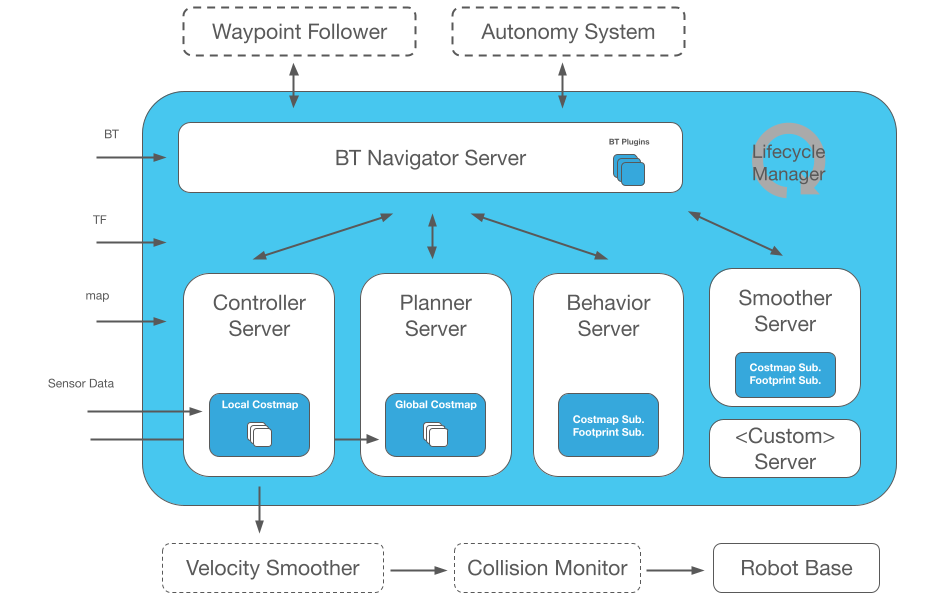
\includegraphics[width=0.8\textwidth]{images/nav2_architecture}
    \caption{Navigation package overview}
    \label{fig:nav2}
\end{figure}

\subsection{Map Server}

This package is used to provide \textbf{map} functionalities to \acrshort{ros}. Basically, it gives you the possibility to \textbf{load} a map from a file and use it for \acrshort{amcl}, or \textbf{save} it after \acrshort{slam} has been run.

\subsection{\acrfull{amcl}}

\acrshort{amcl} is used to \textbf{localize} the robot on a known \textbf{map} using a 2D laser scanner \textbf{probabilistically}. Firstly, once the map is loaded, the initial robot pose \textbf{must be set}\footnote{\acrshort{rviz} lets you set the initial robot pose graphically}: what is going on under the hood is publishing a \code{map} $\rightarrow$ \code{odom} transformation so that the \code{odom} $\rightarrow$ \code{base\_link} one leads to the \textbf{real position} of the robot.

\subsection{\acrfull{slam}}

It is a collection of techniques used to \textbf{localize} and \textbf{map} the environment \textbf{simultaneously}, using 2D laser scans \cite{slam}. Once the map is completely built, it is possible to save it to a file and pass it to the Map Server.

\subsection{Recoveries Server}

It is responsible for executing simple controlled robot movements, like backing up, rotating and stopping when \textbf{recovery} is needed, like when the robot \textbf{hits} something.

\subsection{\acrfull{btnav}}

This one makes use of \textbf{behavior trees} to define the actions to be performed when the robot is in a certain \textbf{state}: for example, when no problem has met, it will continue to navigate and reach the current goal, but when it hits something, the behavior tree will execute the recovery action.

\begin{figure}[h]
    \centering
    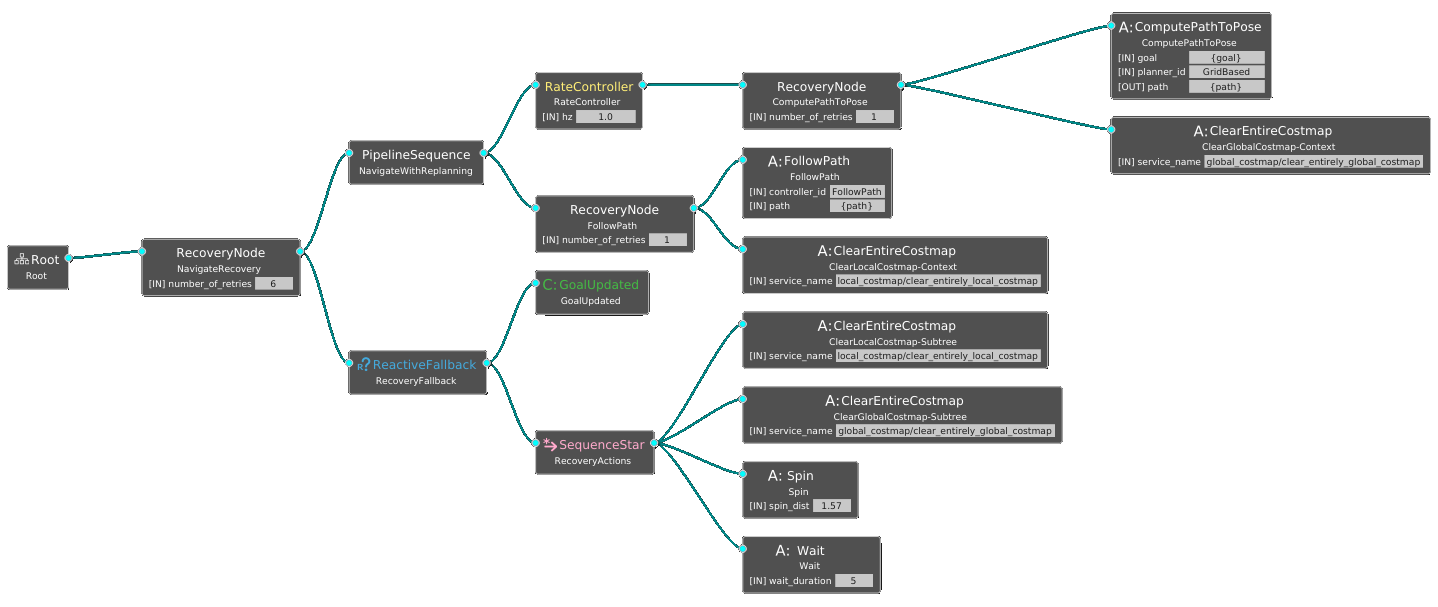
\includegraphics[width=0.9\textwidth]{images/bt-alpha.png}
    \caption{Currently used behavior tree. Groot lets you visualize it, also in real-time. \cite{groot}}
\end{figure}

\subsection{Planner Server}

It implements behavior trees to \textbf{compute path to pose}; it is also possible to choose which pathfinding algorithm you want to use.

\subsection{Controller Server}

It generates \textbf{command velocities} for the wheels using computed path from Planner Server and send them to the robot.

% \subsection{Waypoint Follower} 

% Instead of just setting a single goal, it is possible to navigate a list of waypoints the robot has to pass through. When a waypoint is reached, some plugins can be attached in order to make the robot take a photo, wait for external command or simply wait. Currently, this feature has not been used in the project, because even if multiple rooms are requested to be visited, the planner will only generate subsequent tasks, passing them one by one, after the previous one has been completed.

\subsection{Lifecycle Manager}

All the previous nodes interface with \textbf{Lifecycle Manager}, which brings \acrshort{ros}2 \textbf{managed nodes}\footnote{\textit{A managed life cycle for nodes allows greater control over the state of ROS system. [...] a managed node presents a known interface, executes according to a known life cycle state machine, and otherwise can be considered a black box.} \cite{lifecycle}} concept to the navigation stack: in such a manner, before nodes begin their execution, it \textbf{checks} if all of them were \textbf{launched correctly} and are ready to start, to avoid unexpected behaviors.

\begin{figure}[h]
    \centering
    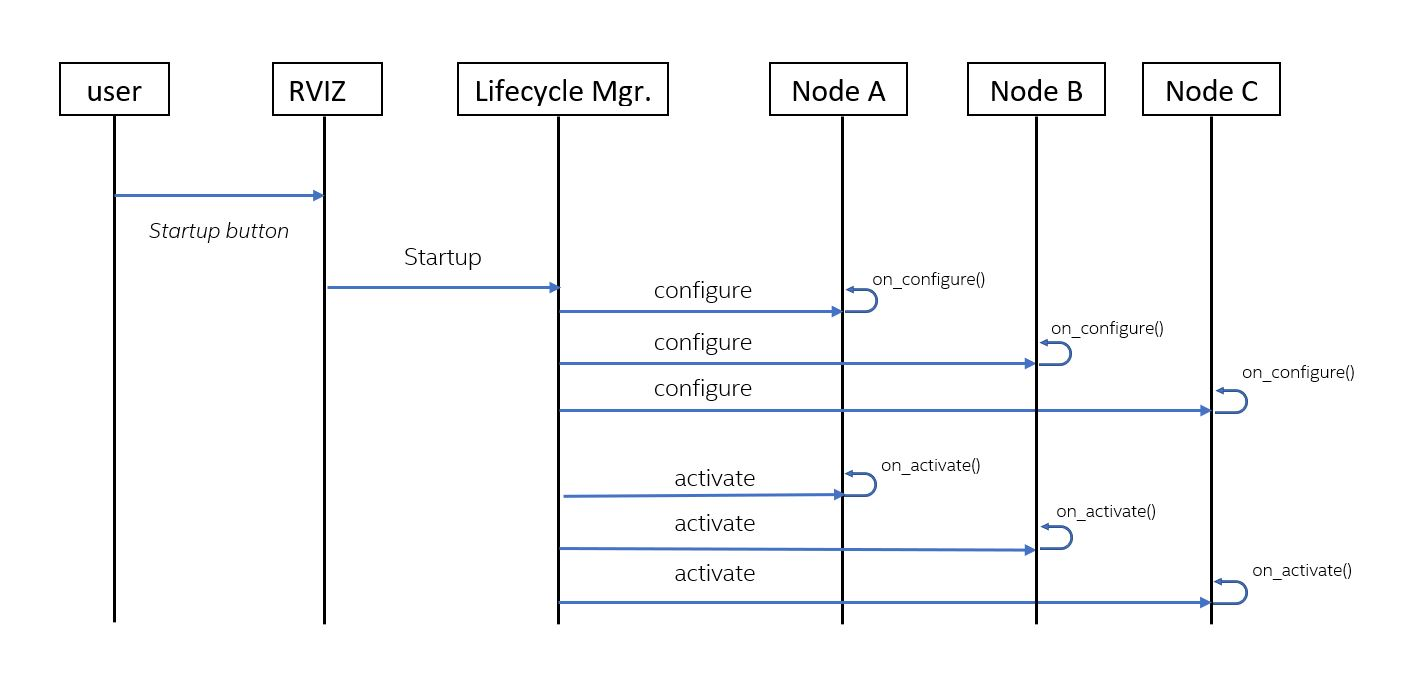
\includegraphics[width=0.8\textwidth]{images/uml_lifecycle_manager}
    \caption{Sequence of service calls when startup is requested}
\end{figure}

\section{\code{ground\_robot\_navigation} package integration}

\begin{wrapfigure}{l}{0.35\textwidth}
    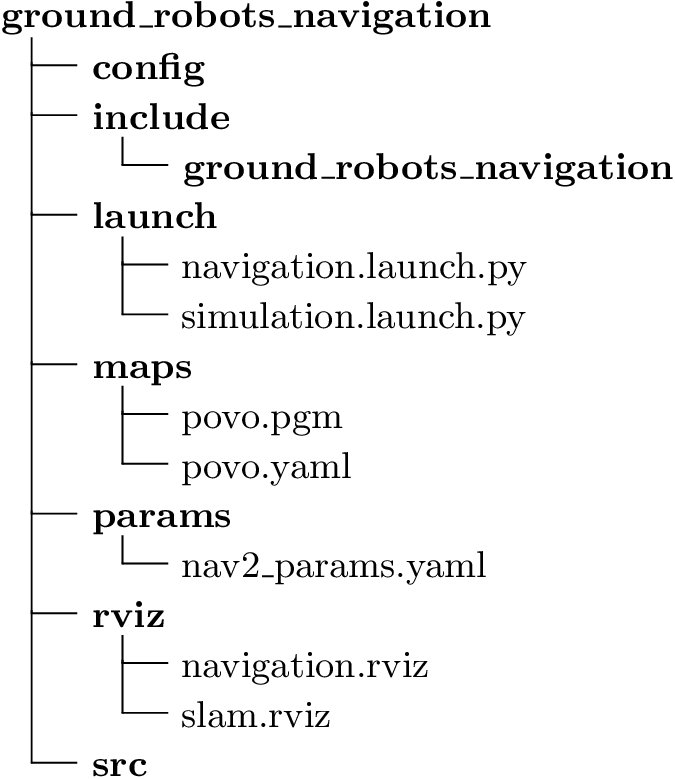
\includegraphics[width=0.35\textwidth]{images/nav_folder}
    \caption{Navigation folder}
\end{wrapfigure}

Everything required to navigating through the environment is provided by \code{ground\_robot\_navigation} package. The complete structure is shown in \autoref{fig:folder}

% TODO: sistemare folder structure (togliere v2 da urdf e aggiugnere "..." se una cartella contiene altri file; sistemare altezza lidar? 0.45 invece di 0.41 come su shelfino?)

Regardless if the robot is real or simulated, there are always a \code{scan}, \code{odom} and \code{cmd\_vel} topic and a \code{map}, \code{odom} and \code{base\_link}\footnote{All the other links of the robot are connected to the last one, the root one} frame. What is still missing is a way to pass this information to \acrshort{nav2} and here comes \code{ground-robot} package, designed specifically for this project.

Inside \code{\acrshort{rviz}} folder there are two \textbf{configuration files} which are going to be loaded when the program starts executing: in the \textit{\_real} one, only some link/joint names are \textbf{missing} because they are no longer simulated and there are no such frame transformations. % check se ne basta uno o no (?)

Folders like \code{include} or \code{src} are left even if empty in the project folder, because it is possible to \textbf{integrate custom algorithms} inside the \acrlong{nav2}, thanks to \code{nav2\_core} package. The same applies for \code{config} one, where you can put your own configuration files, how it was done originally when using \acrfull{ekf} to estimate robot odemetry\footnote{Later removed because of its buggy behavior}, fusing multiple sensors.

\code{params} folder contains the parameters file described in the beginning of \autoref{cha:navigation}.

Inside the \code{launch} folder there is the script used to \textbf{start} the entire \textbf{navigation system}; normally it launches the version with \textbf{real} environment and robot. Here follows a list of the possible arguments you can pass as $<$name$>$:=$<$value$>$ pairs: % (?)

\begin{itemize}
    \item \arguments{use\_namespace/namespace}{whether to apply a namespace and its name}
    \item \arguments{autostart}{if \acrshort{nav2} should be automatically started}
    \item \arguments{slam}{whether to run \acrshort{slam}}
    \item \arguments{params\_file}{full path to parameters file to use for navigation nodes}
    \item \arguments{bt\_xml\_filename}{full path to the behavior tree xml file to use}
    \item \arguments{map}{full path to map file to load}
    \item \arguments{use\_simulator}{whether to start the simulator}
    \item \arguments{headless}{whether to execute Gazebo client \acrshort{gui}}
    \item \arguments{use\_sim\_time}{whether to use simulation time, starting from zero}
    \item \arguments{use\_robot\_state\_pub}{whether to start the robot joint state publisher}
    \item \arguments{world}{full path to the world model file to load}
    \item \arguments{use\_rviz}{whether to start \acrshort{rviz}}
    \item \arguments{rviz\_config\_file}{full path to the RVIZ config file to use}
    \item \arguments{model}{full path to robot urdf file for \acrshort{rviz}}
\end{itemize}

\bigskip

If you want to start a simulation, just set \code{use\_simulator} to \textit{true} and change \code{rviz\_config\_file} path; if you want to \textbf{disable} the \acrfull{gui} of Gazebo, set also \textbf{headless} to \textit{true}.

% parlare di velocità lineare e angolare
% odom su simulazione
% sostituire base_laser con lidar_link e provare a lasciare i joint rimossi (?)